%\documentclass[twocolumn,showpacs,preprintnumbers,amsmath,amssymb,aps,prb]{revtex4-1}

\documentclass[preprint,showpacs,preprintnumbers,amsmath,amssymb,aps,prb]{revtex4-1}

%\usepackage[colorlinks, allcolors=blue]{hyperref}

\usepackage{amsmath}
\usepackage{graphicx}
\usepackage{amsthm}
\theoremstyle{remark}
\newtheorem{problem}{Problem}

\begin{document}

%DM replace?
%\title{Molecular dynamics simulation of synchronization in driven particles}
\title{Molecular dynamics simulation of a driven synchronized particle}

\author{Tiare Guerrero}
\email{guer9330@pacificu.edu}
\affiliation{Department of Physics, Pacific University, Forest Grove, OR 97116}

\author{Danielle McDermott}
\email{mcdermott@pacific.edu}
\affiliation{Department of Physics, Pacific University, Forest Grove, OR 97116}

\date{\today}

\begin{abstract}
  Synchronization
  plays an important role in many physical processes.
  We discuss a 
  molecular dynamics simulation
  of a single particle
  moving through
  a viscous liquid
  while being driven 
  across a washboard potential energy landscape.
  Our results show many dynamical patterns
  as the landscape and driving force are altered.
  For certain conditions,
  the particle velocity and location
  are synchronized or 
  phase-locked,
  forming closed orbits in phase space.
  Quasi-periodic motion is common, 
  for which the
  dynamical center of motion shifts the
  phase space orbit.
  This synchronized motion
  is
  observed in 
  simulations and table-top experiments,
  and
  can be used to isolate
  complex natural behaviors.
 %[suggest omitting this sentence. Code not in text. We include molecular dynamics code
 % to simulate and characterize the
  %particle dynamics.] 
\end{abstract}

\maketitle 

\section{Introduction} 
Synchronization is a universal phenomena
in which
individual oscillators change frequency due
to external stimuli.\cite{Pikovsky2003}
The
flickering patterns of
candle flames [DM - the air molecules are oscillating xx is a flame an oscillator? xx]
mediated by temperature fluctuations,\cite{Okamoto2016}
the vibrations of singing wine glasses interacting 
through sound waves,\cite{Arane2009}
and metronomes vibrating through a supporting platform\cite{Jia2015}
are examples of in-phase coupled oscillations. 
Biological systems benefit from cooperative
synchronization --
birds coordinate wing flaps
to optimize energy use during flight,\cite{Portugal2014}
frogs alternate croaking patterns,\cite{Aihara2014}
humans clap in time with music,\cite{Tranchant2016}
and 
at a cellular level, 
neurons simultaneously fire in cardiac muscle\cite{MartinHall1999}
and brain tissue.\cite{Singer1999}
External forcing can cause or regulate 
synchronization. For example, 
an electrical pacemaker 
regulates a heart beat 
and 
a pulsed light modifies the
flashing pattern of fireflies. 

Synchronized phase-locking or mode-locking 
first appeared in the scientific literature
with 
Huygens' 1665 experiments on the
motions of synchronized 
pendula in wall-mounted clocks.\cite{Bennett2002}
A locked-mode is an integer frequency ratio.
In Huygens clocks,
the pendula were observed to swing at the  same rate
in the same direction (1:1 mode) or
opposite directions ($-1$:1 mode).
A 2:1 mode occurs when a simple pendulum four
times the length of another swings with twice the period.

Complex dynamics such as synchronized mode-locking
can be studied with
colloid particles in experiments.
Typical colloids are   
plastic spheres suspended in
de-ionized water or silica beads suspended in organic solvent.
Because 
colloids are large 
and move slowly, the
particle positions 
can be measured in real time 
with an optical camera.\cite{Pertsinidis2001}
Experimental measurements of the
step-by-step dynamics of 
colloids performing phase-locked motions
are useful for
understanding synchronization at a single particle level.\cite{Juniper2015,Juniper2017}

Light is a
tool for manipulating the colloidal environment
to alter synchronization patterns.
Colloids can be trapped
with 
radiation pressure from 
a laser beam.\cite{Ashkin1997}
A colloid centered in an optical trap is 
uniformly bombarded by photons. 
Off-center colloids 
experience a net force
due to uneven photon collisions across
the particle surface.
Depending on the 
location of the particle in the trap,
the radiation pressure either moves colloids toward the center 
or ejects it from the trap.
Diffraction gratings can create
more complex light environments, 
such as periodic patterns of minima
suitable for synchronization studies.\cite{Grier2003}

The model discussed in this paper
resembles an overdamped driven pendulum.
A single particle oscillator
in a potential well is 
like a skateboarder in a half-pipe or
a child on a swing.
A confined oscillator may 
synchronize its location
to the periodic pattern of the external drive,
moving back and forth in time with
the beat,
or moving between substrate minima.
When 
a constant or 
dc drive is applied,
the particle velocity is modulated by 
the potential energy landscape exerted on the particle.  %seen by the particle.
[DM swapped ``seen by'' for ``exerted on'' xx check added wording xx] 
Below some threshold  
the dc force is not strong enough to push the particle
across a potential maximum so the average velocity is zero,
a phenomena referred to as pinning.\cite{Reichhardt2017}
Above the pinning threshold,
a particle subject to a constant
drive force  increases its speed at a rate proportional
to the external drive.  
When the applied force varies periodically,
the ac drive can 
cause the particle to hop back and forth across
the landscape minima.
Many synchronized patterns occur,
controlled by the substrate period,
leading to 
mode-locking,
where the average particle velocity
is fixed for a range of dc drive forces.\cite{Reichhardt2015}

In this paper we discuss numerical simulations 
of the synchronized dynamics
of a confined particle driven over
a washboard shaped potential energy landscape.
We describe
our molecular dynamics model  in Sec.~\ref{sec:MD}.
The model
is easy to simulate yet relevant
to condensed matter systems.
We summarize our results 
including the synchronized motion of a single confined particle
driven across a periodic landscape in 
Sec.~\ref{sec:results}.

In Sec.~\ref{sec:conclusion}
we describe how our results apply 
to physical systems,
such as optically trapped colloids
%charge density waves in dusty plasma
[DM rewrote to better align with conclusion xx added words is this correct? xx]
and superconducting vortices in the presence of periodic pinning arrays.
% and Josephson junctions.
[DM resolved xx Josephson junctions not explicitly mentioned in conclusion, xx] 
We include problems for interested readers 
in Sec.~\ref{sec:problems}.

\section{Simulation}
\label{sec:MD}
We use a classical model for 
studying the dynamics, %xx you only use single particles xx]
using the net force on a particle to calculate
its trajectory.
The particle is confined in a two-dimensional (2D) [DM singular]
simulation of area $A = L \times L$, where $L=46.\bar{6}\,a_0$
where $a_0$ is a dimensionless unit of length.
[DM - yes.  in the simulation we just use $L=46.6$ and the $a_0$ is to satisfy readers unfamiliar with simulation units xx confused about the role of $a_0$ because it and hence $L$ are dimensionless, Is it really the size of a colloid particle, which in the simulation you set to unity?  xx]
The particle %Particle $i$
[DM resolved xx since we are doing non-interacting particles and thus only one particle is moving can we eliminate the subscript $i$? xx]
has
position $\vec{r} = x \hat{x} + y \hat{y}$
and velocity $\vec{v} = d\vec{r}/dt$.
The edges of the system are treated by
periodic boundary conditions,
such that a particle leaving the edge of the system is mapped
back to a position within the simulation boundaries 
by the transformation $x+L \rightarrow x$ and $y+L \rightarrow y$.
We show a schematic of the system in Fig.~\ref{fig:1_landscape}(a).
The units of the simulated variables are summarized in Table~\ref{tab:1}.
%\footnote{To learn more about the effects of temperature on this simulation see Problem~\ref{ex:brownian}, where we study $U_0 \sim k_B T$.}

We confine the particles using a position dependent 
potential energy, called a landscape or substrate.
The landscape is modulated in the $y$-direction
by the periodic function 
 \begin{equation}
   U(y) = U_0 \cos{(2 \pi y / \lambda)},
     \label{eq:ysubstrate}
\end{equation}
where $\lambda=L/N_p$, with $N_p$ equal to the number of periods,
and $U_0$ is a parameter
 that sets the depth of the minima
 with simulation units of energy $E_0$. 
 We plot this function in 
 Fig.~\ref{fig:1_landscape}
 for $N_p = 3$.  In Fig.~\ref{fig:1_landscape}(a) we show 
 the $x$-$y$ plane with a contour plot of $U(y)$ 
 to illustrate
 the 2D potential energy landscape;
 the maxima are colored gray and the minima colored white.
 [DM - switch from red/blue to gray/white - xx make sure that all your figures make sense when printed in b/w xx]

The confining force on the particle [DM removed subscripts] $i$
 is given by
 \begin{equation}
 \vec{F}_{\ell}(\vec{r}) = - \vec \nabla U(\vec{r}). [DM removed ^{\ell}]
 \label{eq:dudr}
 \end{equation}
 %[xx what does the superscript $\ell$ mean? xx]
 where $\ell$ denotes the landscape.
 In Fig.~\ref{fig:1_landscape}(b) we plot  
 $U(y)$ to illustrate how the magnitude
 $|\vec{F}_{\ell}|$ is calculated from the particle position $y$.
 [DM - begrudingly changed - My collaborators and I usually use superscripts for these equations to separate the force superscripts from the particle index subscripts.  This is consistent with the textbook I teach from.  xx suggest that you use subscripts instead of superscripts. We can easily make that change in the next iteration of your manuscript. However, you would need to change the figures, e.g., $\vec{F}_{\rm d}$ $F_{\rm dc}$ $F_{\rm ac}$. One of us didn't like superscripts where he was an undergraduate!  xx]
 
Particles are subject to an external time-dependent driving force
$\vec{F}_{\rm d}(t)$
applied parallel to the $y$-direction.
We model this force as
\begin{equation}
  \vec{F}_{\rm d}(t) = [F_{\rm dc} + F_{\rm ac} \sin(\omega t)] \hat{y},
    \label{eq:drive}
\end{equation}
with 
a constant component $F_{\rm dc}$
and a time dependent component with amplitude $F_{\rm ac}$
with angular frequency $\omega = 2 \pi f$.

The inertia of 
small particles is reduced by interactions
with the fluid particles.\cite{Purcell1977}
We assume 
colloids are
overdamped
so the particles do not accelerate,
that is, they are suspended in a continuous viscous fluid
that dissipates energy supplied externally. 
Newton's second law for an individual particle
is simplified
by the assumption that $\vec{a}$ is zero. 
The overdamped equation of motion for
the velocity $\vec{v}$ of 
an isolated particle is
\begin{equation}
  \eta \vec{v} = \vec{F}_{\ell}(\vec{r}) + \vec{F}_{\rm d}(t).
    \label{eq:motion}
\end{equation}
with friction coefficient $\eta = 1$ in units of $v_0 / F_0$.
%[xx added $v_0$ to table, please check xx] 
The term $-\eta \vec{v}$
is a drag force, which models
energy dissipation due to the fluid. 
We discuss  models for
spheres moving through fluids in 
Problem~\ref{ex:reynolds}. 

The equation of motion provides a direct calculation of the velocity
of an individual particle at position $\vec{r}$ 
and simulation time $t$.
The   simulation is controlled by a  loop
which runs to a maximum integer time step.
At each time step
we evaluate the net force on each particle as a function of its position
$\vec{r}(t)$
and then integrate
the equation of motion to move particles
to an updated position.
Because the acceleration is zero,
the integration of the equation of motion
is performed via 
the simple first-order Euler method 
\begin{equation}
  \vec{r}(t+\Delta t) = \vec{v}(t) \Delta t + \vec{r}(t)
    \label{eq:euler}
\end{equation}
for a time step $\Delta t = 0.1\,\tau$.
In 
Problem~\ref{ex:euler}
we describe 
the numerical methods for 
solving differential equations.
%------------------------------------------------------------------
\begin{figure} % [h!]
\centering
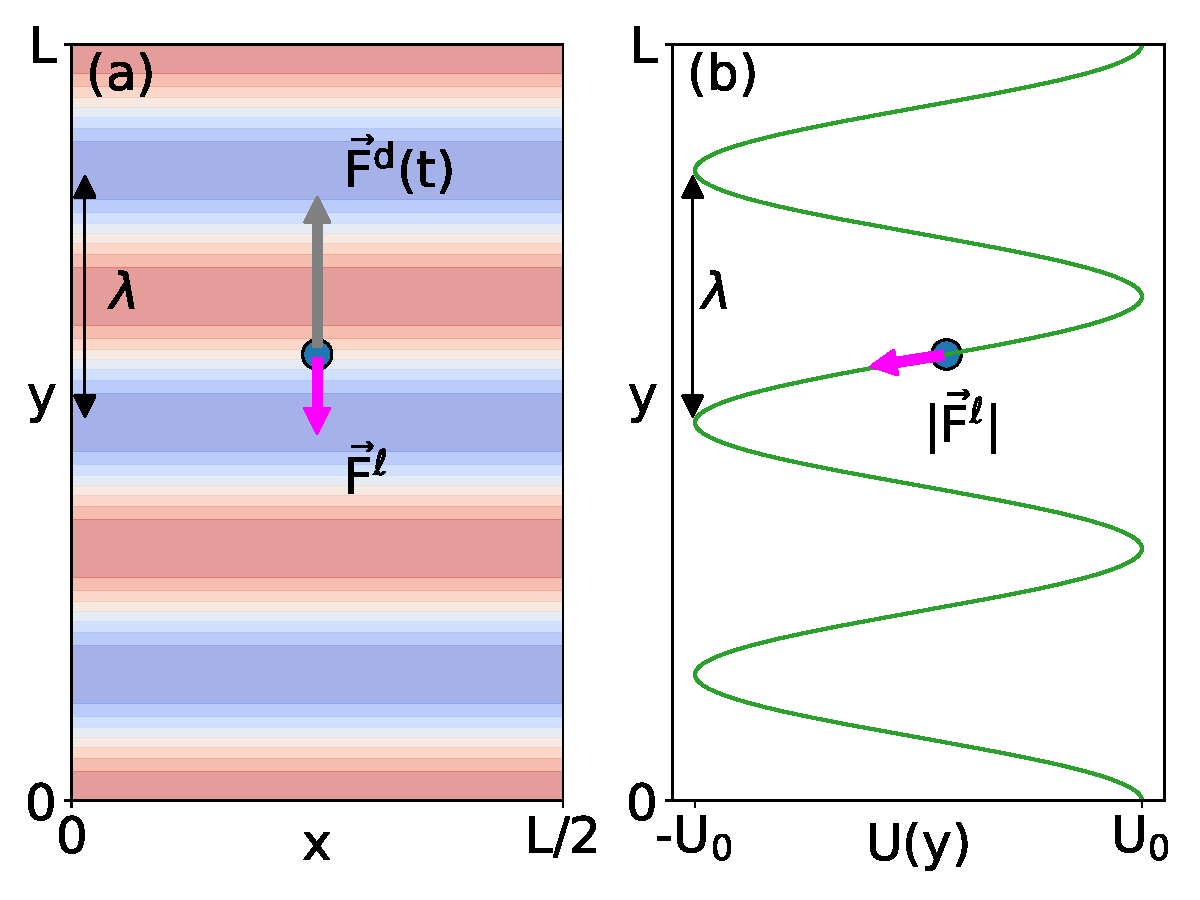
\includegraphics[width=\columnwidth]{fig1_landscape.pdf}
\caption{
Schematic of the simulation of a single particle
  driven across a washboard potential energy landscape.
  (a) View of the $x$-$y$ plane. 
  The time-dependent applied driving force $\vec{F}_{\rm d}$
  is parallel to the $y$-axis.
  The landscape is shown with
  [DM changed color scheme from red/blue to gray/white for better BW conversion]
  maxima in the potential energy are gray %#red
  and minima are white %.
  A particle is 
  subject to competing forces of the landscape and applied driving force.
  (b) The potential energy function
  along the $y$-axis $U(y)$.  [DM removed $_{\ell}$]
  The particle in (a) is shown at the same $y$-position.
  The slope of $U(y)$ [DM removed $_{\ell}$ use the subscripts with the potential, but will move to superscript xx used subscript here xx]
  is the 
  magnitude of force $\vec{F}_{\ell}$. 
  }
\label{fig:1_landscape}
\end{figure}
%
\section{Mode-locking of a single particle}
% In subsection headings, only the first word is capitalized.
\label{sec:results}
Here we drive 
a single particle 
across the landscape. 
The numerical implementation of the landscape 
is calculated with Eqs.~\eqref{eq:ysubstrate} and \eqref{eq:dudr}  [DM - right, two negative signs, one from the derivative, the other from the definition of force.  I found the ``mistakenly'' dropped minus sign in the depths of january and added it.  xx but you should get a + sign not a minus sign xx] 
\begin{equation}
  \label{eq:force}
  {F_{\ell}}_y(y) = A_{p} \sin{(2 \pi y / \lambda)},
\end{equation}
where the force is scaled by the parameter $A_{p} = 2\pi U_0/\lambda$.
In this section we fix the landscape parameters
to $A_{p} = 0.1\,F_0$ 
with $N_p=20$ minima, 
corresponding to a spatial period $\lambda = 2.3\,a_0$.
The competition between the driving force and the landscape potential
can produce a variety of hopping patterns in the particle motion. 
The relative values of $F_{\rm ac}$, $F_{\rm dc}$ and $A_p$
control the rate and distance a  particle moves 
forward and backward in the landscape.
If $F_{\rm d}(t) > A_p$, a particle can 
overcome the barrier height of the landscape,
and 
the particle hops between minima in the energy landscape.
If the driving frequency is low,
as in Fig.~\ref{fig:2_Fd_vy_time},  
the driven particle 
moves 
in a pattern 
with the same frequency 
as the time-dependent force $F_{\rm d}(t)$,
but is modulated by the landscape period.
We explore changes in the frequency and different values of $F_{\rm ac}$ 
in Problem~\ref{ex:parameters}.
Here we vary $F_{\rm dc}$ 
while holding the remaining parameters fixed.

%xx AJP does not use footnotes
\begin{table}[h!]
\centering
\caption{Simulation parameters and units with comparable
  experimental values.~\cite{Juniper2015,Juniper2017} The substrate is scaled by our force units, while an experimental landscape is scaled by the Brownian motion of the particles.  }
\begin{ruledtabular}
\begin{tabular}{c c c } 
Quantity & Simulation Units & Experimental values\\
\hline
length &  $a_0 = 1$ & $ a_0 \sim 1.5 \mu m$\\
energy & $E_0 = 1$ & \\ %$ < E_0 <$ \\
%electric potential & $V(r_{ij}) = E_0/r_{ij}$ \\
%energy & $E_0 = q^2{Z^*}^2/4\pi \epsilon \epsilon_0 a_0$ \\
%dimensionless interaction strength & $q$ \\
%effective colloidal charge & $Z^*$ \\
%solvent dielectric constant & $\epsilon \epsilon_0$\\
force & $F_0 = E_0 / a_0$ & \\ %$<F_0<$\\
time &  $ \tau = \eta a_0 / F_0 $ & $ \tau \sim 3$\,s\\
velocity &  $ v_0 = a_0 / \tau $ &  $v \sim 5\,\mu$m/s \\
%driving period & $T = 100 \tau$ & $T \sim 1.3$ s \\ %frequency 0.75 Hz
%juniper uses water–ethanol mixture
substrate period & $\lambda = 2.3\,a_0$ & $\lambda = 3.5\,\mu$m \\
substrate amplitude & $A_p = 0.1\,F_0$ & $U_0 = 25 k_B T \sim 1\, {\rm J}$ \\ %$U_0 = 0.037 E_0$ 
temperature & $T_0 = 0$  & $T \sim 290\,$K  \\
\end{tabular}
\end{ruledtabular}
\label{tab:1}
\end{table}

In Fig.~\ref{fig:2_Fd_vy_time}(a)
we plot $F_{\rm d}(t)$ 
as a function of time with the
constants $F_{\rm dc}=0.07$, 
$F_{\rm ac}=0.07$ and $f=0.01$ cycles per time unit $\tau$.
The temporal period of the driving force is
$T = 1/f = 100\,\tau$.
In Fig.~\ref{fig:2_Fd_vy_time}(b) 
we show the $y$-position of the particle
as a function of time,
where we have
normalized $y$ by $\lambda$.
The initial particle position is $y = 0$. 
The particle moves
in the positive $y$-direction
through a distance $\Delta y = \lambda$  in a time $T$,
so that  
the average velocity 
$\langle {v}_y \rangle = \lambda f$. 
The inset of Fig.~\ref{fig:2_Fd_vy_time}(b)
shows $y$ 
over one period $100\,\tau < t < 200\,\tau$
with 
the contour plot described
in Fig.~\ref{fig:1_landscape}(a).
The motion is synchronized such that the 
driving force is a maximum when the landscape 
force is minimum,
as shown by the coincidence of the
steep slope of 
$y/\lambda$ 
and the maxima in $F_{\rm d}(t)$.
When $F_{\rm d}(t)$ is large,
the particle moves across the substrate maxima,
[DM - color change]
shown in gray with the contour plot.
%DM commented out - too much detail
%The slope of $y/\lambda$ equals zero twice
%during a driving period,
%indicating zero
%forward motion 
%due to a coincidence of the negative
%driving force and motion over the landscape maxima.
%------------------------------------------------------------------------
\begin{figure}[h]
\centering
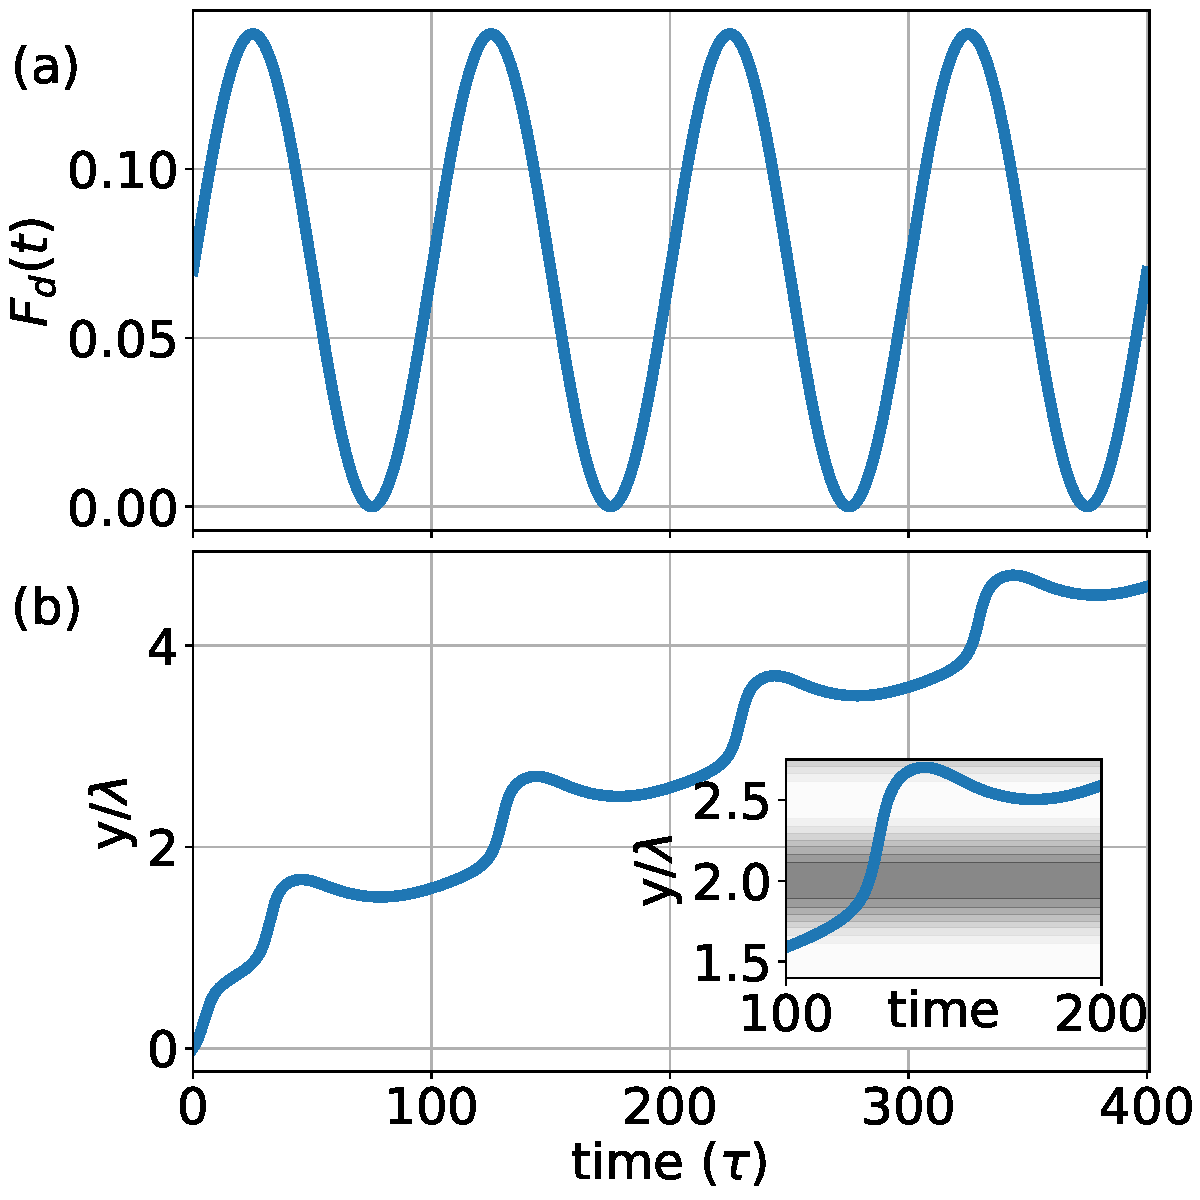
\includegraphics[width=\columnwidth]{fig2_Fd_vy_time.pdf}
\caption{(a) The applied driving force $F_{\rm d}(t)$ 
  with parameters $F_{\rm dc} = 0.07$, $F_{\rm ac} = 0.07$ and $f=0.01$.
  (b) 
  The $y$-position of the driven particle
  normalized by the period of the substrate $\lambda$.
  The substrate strength is $A_p=0.1$.
  The inset   shows
  the $y$-position
  through the second period $100\tau<t<200\tau$
 along with the contour plot depicting
  the landscape potential described in Fig.~\ref{fig:1_landscape}(a).
  }
\label{fig:2_Fd_vy_time}
\end{figure}

To explore the possible hopping patterns,
we sweep through a range of $F_{\rm dc}$ for fixed $F_{\rm ac}$ and $A_p$.
In Fig.~\ref{fig:3_sweep_vyFDC} 
we increase $F_{\rm dc}$ in increments of $0.001\,F_0$,
and 
measure the average velocity $\langle v_y \rangle $ 
as a function of $F_{\rm dc}$.
We also perform the sweep for a non-oscillatory drive $F_{\rm ac} = 0$.
With no oscillating component of the driving force,
  the force-velocity relation increases monotonically 
  above the depinning threshold $F_c$ such that
  \begin{equation}
    \langle v_y \rangle \propto (F_{\rm dc}-F_c)^{-\beta}.
  \end{equation}
  %[xx what is $\beta$? xx]
  where the power $\beta$ varies with the
  system type and
  can be used to identify universality class. \cite{Reichhardt2017}
  The critical force $F_c$ is equal to the maximum substrate force
  $A_p$.
  
The addition of an ac drive leads
  to the formation of modes.
  A mode is a periodic pattern of hops
  with a constant average particle velocity, $\langle {v}_{y} \rangle$
  over a range of driving forces $F_{\rm dc}$.
  In Fig.~\ref{fig:3_sweep_vyFDC}
  we sweep $F_{\rm dc}$
  with $F_{\rm ac} = 0.07$ and $f=0.01$.
Each step represents a different pattern of hops
between substrate minima
performed by the particle
due to the landscape confinement.  
At 
low $F_{\rm dc}$ the average velocity $\langle v_y \rangle$ is zero.
Because 
$A_p$ is large compared to the extrema of $F_{\rm d}(t)$,
the particle oscillates back and forth
in a single minima with no net velocity, an example of 
a 0:0 mode.
At higher $F_{\rm dc}$ the particle velocity 
$\langle v_{y} \rangle$ increases in steps of uniform height,
$\langle v_{y} \rangle = n \lambda f$,
where $n$ is an integer.
We observe a mode of $n=1$
for the range $0.05 < F_{\rm dc} < 0.08$,
$n=2$ for $0.08 < F_{\rm dc} < 0.11$,
$n=3$ for $0.12 < F_{\rm dc} < 0.13$,
$n=4$ for $0.14 < F_{\rm dc} < 0.155$, and 
$n=5$ for $0.155 < F_{\rm dc} < 0.16$.
Higher modes are not visible.
The step width is nonlinear
and depends on the strength of $F_{\rm ac}$
%as a Bessel function 
for this landscape potential.\cite{Reichhardt2000,Juniper2017}
%[DM the step width - simply removed xx what quantity depends on a Bessel function? xx]
These steps, known as Shapiro steps, can have a variety of
interesting patterns
such as a devil's staircase related to chaotic dynamics.\cite{Bak1986}

\begin{figure}[h]
\centering
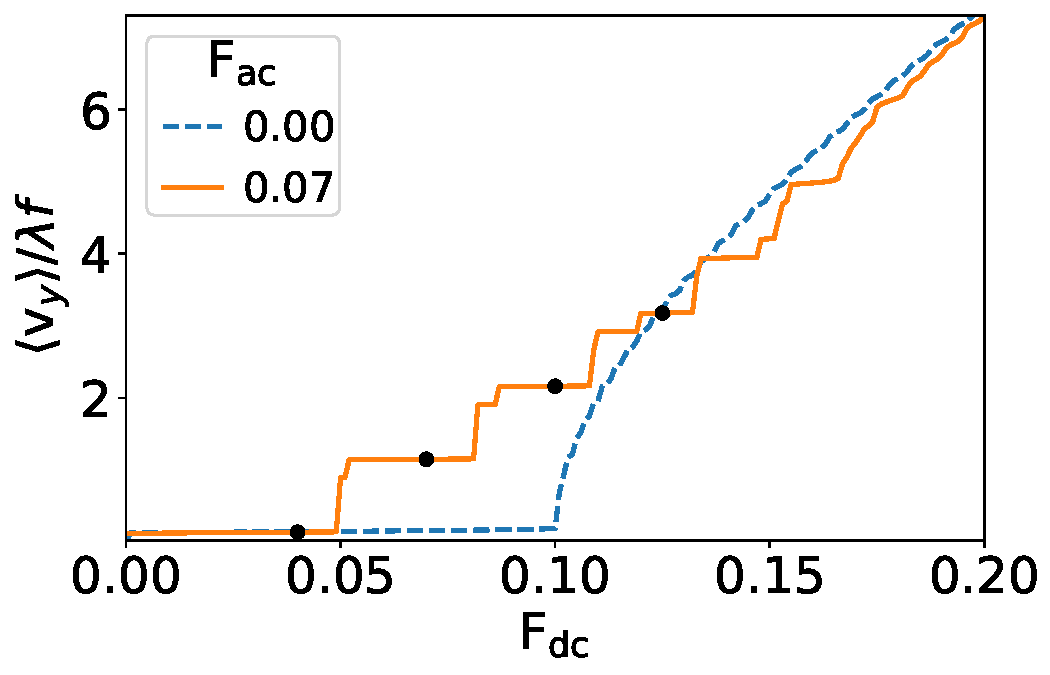
\includegraphics[width=\columnwidth]{fig3_sweep_vyFDC.pdf}
\caption{Average particle velocity  $\langle v_{y} \rangle$
  as a function of $F_{\rm dc}$.
  We let
  $F_{\rm ac}=0.0$ (blue dashed) and 
  $F_{\rm ac}=0.07$ (orange) with $f = 0.01$ 
  as in Fig.~\ref{fig:2_Fd_vy_time}.
  The value of $F_{\rm dc}$ for the first four steps
  %is given,
  correspond with the fixed value of $F_{\rm dc}$
  in each of the phase plots
  %indicating a system
  in Fig.~\ref{fig:4_phase}(a-d).
  [DM - clarified?  xx don't understand meaning of indicating a system
  plotted in Fig.~\ref{fig:4_phase} xx]
}
\label{fig:3_sweep_vyFDC}
\end{figure}

  To study synchronization patterns, 
  it is useful to compare
  mode-locked quantities 
  in a two-dimensional phase plot. 
  For a driven pendulum confined to a single potential well,
  an appropriate
  phase space is the particle velocity $v_y$ versus the position $y$.  
  For a particle driven 
  through multiple identical wells 
  we define phase variables 
  to account for the net increase in the position.
  The phase position is
  \begin{equation}
    \phi(t) = 2\pi [y(t)-\langle v_y \rangle t]/\lambda,
  \end{equation}
  centered about the average particle displacement $\langle v_y \rangle t$
  and normalized by the substrate period $\lambda$.\cite{Juniper2015}
  The phase velocity is
  \begin{equation}
    \dot{\phi}(t) =2\pi [v_y(t)-\langle v_y \rangle] /\lambda.  
  \end{equation}
  For zero landscape force, 
  the phase velocity  is zero when $F_{\rm d}(t) = F_{\rm dc}$.
  [DM rewrite following sentence]
  If the system
  is strictly mode-locked,
  the particle velocity
  recurs at a particular spatial location, and 
  %If the velocity
  %is mode-locked to 
  %a spatial location,
  %[xx don't understand meaning of the velocity
  %is mode-locked to 
  %a spatial location xx]
  a closed loop appears in  
  phase space. 
  A 1:1 mode appears as a circle or oval. 
  Nodes appear 
  for higher modes,
  sometimes forming figure-eights
  or other recognizable patterns.
  A system that is nearly phase locked
  will appear as an almost closed loop.
  Such quasiperiodic systems are
  not fully synchronized
  so the position-velocity relation
  shifts in time as in Fig.~\ref{fig:4_phase}.
  
  In Fig.~\ref{fig:4_phase}
  we plot $\dot{\phi}(t)$ versus $\phi(t)$
  for increasing 
  $F_{\rm dc}$, 
  with the remaining parameters fixed as in Fig.~\ref{fig:2_Fd_vy_time}.
 %[xx this sentence not helpful, what is plotted is clear: For clarity the plots are normalized by the prefactor $2\pi$.  xx]
  For
  $F_{\rm dc} = 0.04$
  the phase plot   in Fig.~\ref{fig:4_phase}(a) with is an
  % small [xx not clear what small means? can we eliminate this word? xx]
  asymmetric curve.
  A tail appears
  due to the initial transient
  motion of the particle.
  The particle is confined to a single
  substrate minima,
  and has no net velocity.
  The asymmetry is caused by bias induced by $F_{\rm dc}$.
  In Fig.~\ref{fig:4_phase}(b)
  with $F_{\rm dc} = 0.07$
  the phase loop is a symmetric triangular shape,
  indicating a 1:1 match between the
  particle motion and velocity consistent with 
  Fig.~\ref{fig:2_Fd_vy_time}(a).
  As $F_{\rm dc}$ is
  increased,
  nodes form in the phase diagram, which
   occur due to repeated values
  of $\dot{\phi}$ over multiple phase positions.
  In Fig.~\ref{fig:4_phase}(c)
  with $F_{\rm dc} = 0.1$
  two nodes form.
  The particle moves a distance $2\lambda$
  during one time period.
For $F_{\rm dc} = 0.125$ as in Fig.~\ref{fig:4_phase}(d),
  three nodes form as the particle moves across $3\lambda$.
  
    \begin{figure}[h!]
      \centering
      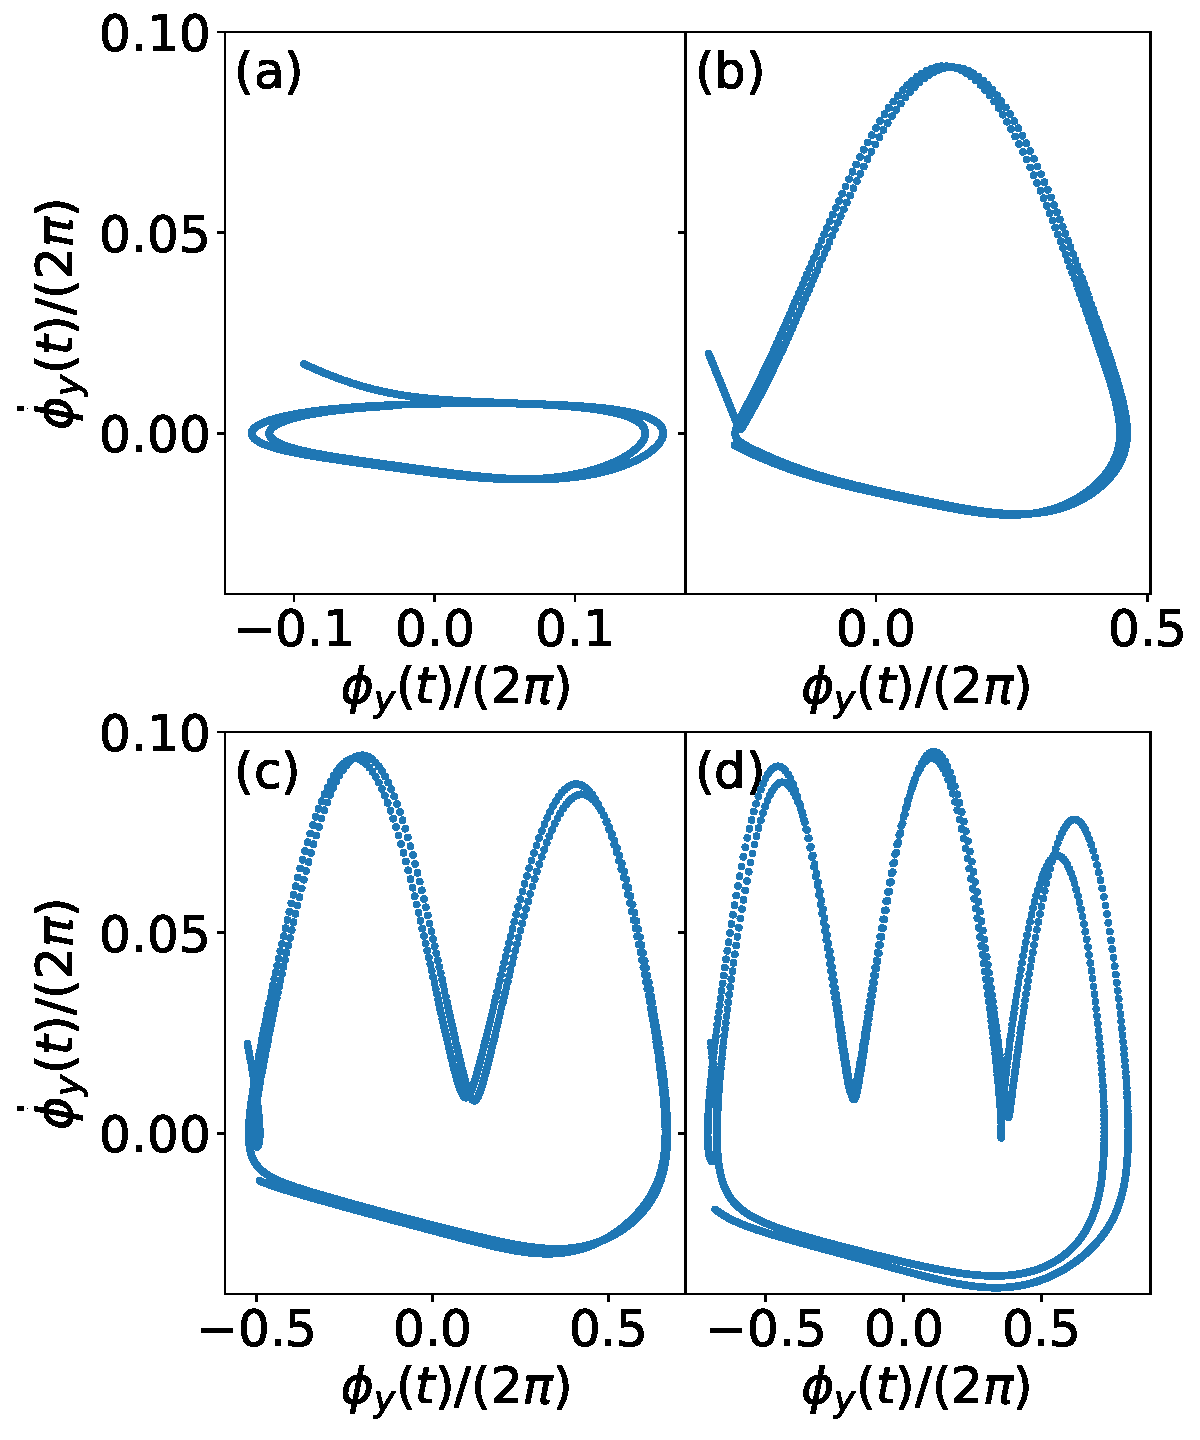
\includegraphics[width=\columnwidth]{fig4_phase.pdf}
      \caption{
        Phase plot of $\dot{\phi(t)}/(2\pi)$ versus $\phi(t)/(2\pi)$.
        The particle is driven with $F_{\rm dc}$ equal to  (a) $0.04$, (b) $0.07$, (c) $0.1$, and (d) $0.125$.  These values are denoted as black circles
        in Fig.~\ref{fig:3_sweep_vyFDC}. 
      The other parameters
      are $F_{\rm ac} = 0.07$, $f=0.01$, and $A_p = 0.1$
      as in Fig.~\ref{fig:2_Fd_vy_time}.}
      \label{fig:4_phase}
    \end{figure}

\section{Conclusion}
\label{sec:conclusion}	
A single particle driven across a periodic potential landscape 
synchronizes its motion 
to environmental and external forces.  
Our simulations reproduce the experiments and simulations presented in 
Juniper {\it et al.} \cite{Juniper2015, Juniper2017}
of 
mode locking in
driven colloids on a
periodic optical landscape.
Colloids are 
relatively easy to 
manipulate and image in experiments,
making ideal proxies 
for systems 
such as cold atoms or electron gases.\cite{Grier2003}
Dynamical mode-locking 
is 
observed in  technologies such as 
 quantum electronic
devices as 
stepped regions in the relation between current-voltage,
where the voltage is the analog of the external driving force
and current is the analog of particle velocity.
These mode-locked or phase-locked currents (Shapiro steps), 
due to applied ac voltages in 
single Josephson junctions\cite{Shapiro1963, Golubov2004} and
coupled arrays of junctions have been observed.\cite{Benz1990}
Shapiro steps vary in width depending on the strength of the
applied ac forces,
and are observed in a variety of ac and dc driven systems
displaying
non-Ohmic behavior in voltage-current curves,
including
charge density waves, spin density waves
and superconducting vortices in landscapes 
engineered with periodic patterns of pinning sites.\cite{Reichhardt2000}

Mode-locking is a useful probe 
of complex quantum mechanical systems
because the motions of individual particles can  be inferred only
from other measurements.
Our results are relevant 
to synchronization effects
in a broad range of experimental systems
including optically confined colloids,
superconductors with periodic pinning arrays, 
and the charge and spin of atomic systems.

\section{Suggested problems}
\label{sec:problems}	

In the following
we explore the behavior of our model
with suggested problems for interested readers.
We discuss the molecular dynamics algorithm
and
numerical integration techniques in Problem~\ref{ex:euler}.
[DM slight rewrite to remove the redundant ``we'' active voice construction]
Changes to the parameters are described in 
%We explore changes in the particle motion
%with parameter changes in
Problem~\ref{ex:parameters}.
We include analytic solutions to  the 
linear drag equation in Problem~\ref{ex:reynolds}, 
the equation of motion in Problem~\ref{ex:n2l}.
%[DM working on it xx see comment below xx]
%DM rewrite of the following sentence - unclear as written/edited
We extend the numerical model %with
%numerical problems 
to include finite temperature effects
in Problem~\ref{ex:brownian}.

\begin{problem}{Write your own MD code}
  \label{ex:euler}
  %[xx you didn't really discuss other integration algorithms, you just mentioned some names That's OK. Instead you might want to make this problem 1 and guide readers to write their own program. Then mention that a program is available, which you only mention in the abstract xx]
  To calculate the position of the particle
  %DM add
  as a function of time
  %DM end
  we
  numerically integrate the equation of motion
  %DM add
  (Eq.~\ref{eq:motion})
  %DM end
  using
  the standard definition of velocity
  $\vec{v} = d\vec{r}/dt$ 
  using the 
  Euler method.
  %DM substituted direct reference for ``The equation of motion...''
  Eq.~\ref{eq:motion} provides
  a direct calculation for the particle velocity
  from the net force on the particle,
  as demonstrated in Problem~\ref{ex:n2l}.

    A working example of this code is available
  in Ref.~\cite{supplemental}
  If you would like to write your own,
  the following guide
  will walk you through our choices.
  In the code excerpts below,
  most comments and optional details are removed for clarity.
    %The molecular dynamics
  %described above
  %is available in Ref.~\cite{supplemental}
  We use the Python programming
  language
  for educational purposes.
  To model additional particles,
  the authors recommend a more traditional 
  compiled coding language
  to perform the many operations associated
  with neighbor lists to compute particle interactions.
  
  \begin{enumerate}
    
  \item[(a)] {\bf Initialization.}
    For convenience,
    we define a Python dictionary
    to contain the simulation constants
    that could easily be passed by reference
    to subroutines.
    We have left as an exercise to the reader the addition
    of the remaining parameters of the system.
    \begin{verbatim}
def set_parameters():           
    ```set simulation parameters...'''

    #declare the dictionary     
    dict={}  
    dict[`dt'] = 0.1 #timestep in simulation units
    #control the oscillating component of driving force
    dict[`F_AC'] = 0.07 #amplitude of force oscillation
    dict[`freq'] = 0.01 #frequency of force oscillation
    #left as an exercise to the reader
    #...
    return dict

    \end{verbatim}

    The function is called at the top of the main function
    followed by a call to a subroutine
    containing the MD algorithm.

     \begin{verbatim}
    if __name__ == "__main__":
        parameters = set_parameters()
        #run the MD simulation
        single_particle(parameters)

\end{verbatim}

    
   \item[(b)] {\bf Time loop.}
     The Euler method is effective
     for solving linear ordinary differential  equations
     of the form
     $dy/dt = f(t,y(t))$ with the initial condition $y(t_0) = y_0$.
     The solution is calculated algorithmically
     by stepping in time through $n$ integer steps
     $t_n = t_0 + n \Delta t$.
     At each subsequent step the new
     value for $y$ is calculated as a  solution of a map using
     discrete times 
     $y_{n+1} = y_n + f(t_n,y_n)$.
     Apply the Euler method to %our equation of motion
     Eq.~\ref{eq:motion}
     [DM - resolved xx refer to specific equation by label xx]
     to determine  the analytic expression
     for the position of a particle
     $y_n$ at the $nth$ time step.
  
     Add a $for$ loop
     to step through each integer timestep.
     With this loop, 
     control
     the flow of the program
     and retain information for the particle position and other
     properties
     as a function of time.
     Assume this information
     will be calculated a subroutine.
        
     We used the subroutine {\bf single\_particle()}
     calculate the array lengths to hold
     position, velocity, and time data.
     The lengths of these arrays will be affected by
     how much data you choice to save
     (see comment following sample code).
     Define a loop to 
     calculate the particle position and velocity through each
     molecular dynamics time step,
     calculated in the subroutine {\bf md\_step()}
     which will be described in more detail in (c).

\begin{verbatim}
def single_particle(parameters,plot="y-position"):
    ```Run MD simulation...'''    
    #define empty arrays to hold data as a function of time
    #(left as an exercise to the reader)   

    #loop through the integer time steps in the simulation
    for int_time in range(0,maxtime):
        #(left as an exercise to the reader)
        time += dt
      
\end{verbatim}

{\it Comment:}     
     A key decision for any MD algorithm
     is how much information to save during and after
     the simulation.
     %DM if going to emphasize this, have the reader do something with it
     %cut out - and make a comment rather than a statement going nowhere
     We define the following constants
     to manage the length of arrays
     containing data.
     We found in practice that for 
     short simulations times
     we could save all data.

\begin{verbatim}
#integer time steps
dict[`maxtime']=int(40/dict['freq'])   #total time steps 
dict[`writemovietime']=1   #write data to arrays for plotting
\end{verbatim}
%dict['decifactor'] = 1     #decimation factor - when to average values 

\item[(c)] {\bf Position and force calculations.}
  %[DM moved sentences about general numerical solution to beginning
  %and those about time to (b)]
  In our implementation,
  we created a subroutine to consider each
  type of force in the system (external drive, landscape, etc).
  If the particle moves beyond the limits
  $0 \le y < L$,
  it must be returned 
  using the definition of periodic boundary conditions
  in Sec.~\ref{sec:MD}.

\begin{verbatim}
  def md_step(y, int_time, avg_vy, parameters, ft=0):
    ```Calculate net force and integrate eq. of motion...'''

    #calculate the floating point value for time
    time = int_time * dt

    #reset vy for every timestep since ay = 0 
    vy = 0 

    #calculate the net force on the particle
    vy = #(left as an exercise to the reader)

    #calculate the new position
    y += #(left as an exercise to the reader)

    #check periodic boundary conditions
    #(left as an exercise to the reader)

    return y, vy, avg_vy

\end{verbatim}

%  \item[(d)]
    
  \end{enumerate}

  The Euler algorithm can be applied to
  calculate reasonable numerical solutions to 
  nonlinear
  equations if the time step $\Delta t$
  is kept sufficiently small.\cite{Newman}
  In our simulations we use the time step $\Delta t = 0.1$
  and find no change in the solution
  when we decrease the time step to smaller values.
  In simulations of
  many interacting particles,
  a small
  time step is essential for accurate results.
  Particle-particle interactions are typically nonlinear,
  so that the interparticle force changes significantly over small distances and the simple Euler algorithm is insufficient.
  
\end{problem}

\begin{problem}{Exploring model parameters}
\label{ex:parameters}

\noindent A range of oscillation behaviors
can be explored by varying the
  relative strength of the confining landscape
  and the external driving force.

\begin{enumerate}

\item[(a)]
  Explore the effect of increasing $F_{\rm ac}$ on the hopping pattern.
  For a single driven particle,
  the hopping patterns are typically characterized
  by $n_f$, the number of forward steps,
  versus $n_b$, the number of backward steps  in one
  time period.
  The total displacement of $(n_f - n_b) \lambda$ 
  is the net hop length.  
  In Fig.~\ref{fig:2_Fd_vy_time},
  the particle moves forward through a minima ($n_f = 1$),
  and does not move backward through a full minima ($n_b = 0$).  
  To achieve
  backward hops,
  the driving parameters must have
  a ratio of $F_{\rm ac}/F_{\rm dc} > 1$ 
  and a difference $|F_{\rm ac} - F_{\rm dc}| > A_p$.
  Holding all other parameters fixed,
  explore how the hopping pattern
  changes for increasing $F_{\rm ac}$.
  For example,
  calculate the patterns of hops for
  fixed parameters 
  $f=0.01$, $F_{\rm dc}=0.07$, and $A_p = 0.1$
  and
  modified parameter
  $F_{\rm ac} = 0.2, 0.3$ and $0.4$.
  
  %In Ref.~\onlinecite{Juniper2015}
  %experiments with single colloids 
  %produce 
  %the following
  %combinations of forward and backward steps
  %by sweeping through
  %a variety of applied forces parameters $F_{\rm dc}$ and $F_{\rm ac}$:
  %$n_f = 0$ to $6$ for $n_b = 0$,
  %$n_f = 0$ to $5$ for $n_b = -1$,
  %and
  %$n_f = 2$ to $3$ for $n_b = -2$.
  %In Fig.~\ref{fig:5_Fac_y_vs_time}
  %we fix $f=0.01$, $F_{\rm dc}=0.07$, and $A_p = 0.1$,
  %and increase
  %the amplitude of $F_{\rm ac}$.
  %This increase causes the number of backward steps to increase.
  %The number of forward steps also increases
  %due to the increased total positive amplitude of $F_{\rm d}(t)$.
  %In Fig.~\ref{fig:5_Fac_y_vs_time}(a) 
  %$F_{\rm ac} = 0.2$ %, $0.3$ and $0.4$.
  %the number of backward steps
  %$n_b = 0$ with $n_f = 4$.
  %In Fig.~\ref{fig:5_Fac_y_vs_time}(b) $F_{\rm ac} = 0.4$
  %$n_b = 2$ and $n_f = 6$.
  %In each case the average velocity 
  %is $\langle v_y \rangle = 4\lambda f$,
  %which can be reproduced over a variety of $F_{\rm ac}$ values.
  %[xx what is the question? leave something to the reader! xx]

  %----------------------------------------------------------
  %\begin{figure} %[h!]
  %    \centering
  %    \includegraphics[width=\columnwidth]{{fig5_Fac_y_vs_time}.pdf}
  %    \caption{
%The motion of a particle with the same values of $F_{\rm dc}$ and frequency as in Fig.~\ref{fig:2_Fd_vy_time} and  $F_{\rm ac}$ equal to
%        (a) $0.2$ and
%        (b) $0.4$.
%      }
%      \label{fig:5_Fac_y_vs_time}
%    \end{figure}


\item[(b)] Explore the effect of increasing the driving frequency on the hopping pattern. In Sec.~\ref{sec:results}
  the frequency is sufficiently low so that the effect of 
  the applied force is large
  over a sustained time interval,
  allowing the particle to hop a substrate maxima.
  For example fix
  the parameters
  $F_{\rm dc}=0.1$, $F_{\rm ac}=0.05$, and $A_p = 0.1$
  and explore
  high frequency 
  ($f = 0.1$),
  intermediate frequency 
  ($f = 0.01$),
  and low frequency
  ($f = 0.005$).
  %Figure~\ref{fig:6_freq}
  %shows the effects of increasing the frequency
  %of the applied driving force.
  %The remaining parameters are fixed at
  %$F_{\rm dc}=0.1$, $F_{\rm ac}=0.05$, and $A_p = 0.1$.
  %We observe no backward steps 
  %($n_b = 0$) 
  %across a broad range of frequencies
  %because $F_{\rm dc} - F_{\rm ac}= 0.0$.
  %The rate of forward hops 
  %increases as frequency decreases,
  %but in each case the particle
  %hops across at most one substrate periods as in Fig.~\ref{fig:2_Fd_vy_time}.
  %In Fig.~\ref{fig:6_freq}(a)
  %the high frequency $f=0.05$ suppresses forward motion entirely.
  %The high frequency 
  %is apparent in the undulations of the particle
  %with a period of $20\,\tau$.
  %  
  %In Fig.~\ref{fig:6_freq}(b) the frequency $f= 0.022$
  %with a period of $45\,\tau$
  %arrests the particle between minima,
  %with a hopping rate of seven periods ($320\,\tau$).
  %At an intermediate frequency 
  %such as $f=0.01$,
  %the particles are synchronized so that 
  %the hopping rate matches the driving frequency,
  %as in Fig.~\ref{fig:2_Fd_vy_time}.
  %In Fig.~\ref{fig:6_freq}(c) $f=0.005$
  %the particle hops forward two minima for every period of $200\,\tau$.
  %Low frequencies
  %result in a sustained positive motion of a particle.
  %In Fig.~\ref{fig:6_freq}(e) $f=0.001$
  %the hopping is continuous
  %over the time $100\,\tau < t < 400\,\tau$,
  %with the cycle repeating 
  %over the period length $1000\,\tau$.
  %[xx same comment. too much information xx]
  %
  %\begin{figure} %[h!]
  %  \centering
  %  \includegraphics[width=\columnwidth]{{fig6_freq}.pdf}
  %  \caption{
  %    Motion of a particle with the same values of $F_{\rm dc} = 0.07$ and $F_{\rm ac} = 0.07$ as Fig.~\ref{fig:2_Fd_vy_time} and  frequency $f$ equal to (a) $0.05$, 
  %      (b) $0.022$, (c) $0.005$ and (d) $0.001$. 
  %  }
  %  \label{fig:6_freq}
  %\end{figure}
  %
  %
\item[(c)] Explore the effect of increasing increasing $F_{\rm ac}$ on the step pattern in Fig.~\ref{fig:3_sweep_vyFDC}.
  For example sweep the driving force $F_{\rm dc}$
  over increments of $\Delta F_{\rm dc} = 0.001$
  for a fixed amplitude $F_{\rm ac}$ and frequency $f=0.01$.
  Appropriate values for 
  $F_{\rm ac}=0.1 - 0.4$
  will demonstrate a change in the step width
  in a plot of $\langle v_y \rangle$ vs $F_{\rm dc}$
  
  %In Fig.~\ref{fig:7_sweep2_vyFDC}
  %we sweep the constant driving force $F_{\rm dc}$
  %for a fixed amplitude $F_{\rm ac}$ and frequency $f=0.01$.
  %In the high frequency limit,
  %the regions of phase locking
  %are separated by regions of $F_{\rm dc}$
  %that do not phase lock,
  %and appear to increase linearly with increasing $F_{\rm dc}$.
  %The width of the phase locked steps
  %grows with increasing $F_{\rm ac}$,
  %because 
  %the particle may move backward
  %over a broader range of $F_{\rm dc}$.
  %
  %\begin{figure} %[h!]
  %  \centering
  %  \includegraphics[width=\columnwidth]{{fig7_sweep2_vyFDC}.pdf}
  %    \caption{
  %      $\langle v_y \rangle$ versus $F_{\rm dc}$ of a particle with
  %      $F_{\rm ac}=0.1$ (blue), $F_{\rm ac}=0.2$ (orange),
  %      $F_{\rm ac}=0.3$ (green) and $F_{\rm ac}=0.4$ (red)
  %      with frequency $f=0.01$.
  %      The substrate is as in Fig.~\ref{fig:2_Fd_vy_time}
  %      with $A_p = 0.1$.
  %    }
  %    \label{fig:7_sweep2_vyFDC}
  %  \end{figure}
  \end{enumerate}
  \end{problem}
  
  \begin{problem}{Drag models and Reynolds numbers}
\label{ex:reynolds}

\noindent Stokes' law describes the drag force
  $\vec{F}_{lin} = -3 \pi \eta D \vec{v}$ 
  on a sphere
  moving through a viscous liquid at velocity $\vec{v}$,
  where $\eta$ is the dynamic fluid viscosity and 
  $D$ is the particle diameter.\cite{Taylor2005}
  In simulations we
  subsume the constants $3 \pi D$
  such that $3 \pi D \eta \rightarrow \eta $.
  Often drag forces are
  modeled as a polynomial series\cite{Taylor2005}
  \begin{equation}
    \vec{F}_{\rm drag} = -b \vec{v} - c v^2 \hat{v} + \cdots  .
  \end{equation}
  Truncating the series to the first term
  is justified by demonstrating the sphere
  has a low Reynolds number  
  $R = D v \rho / \eta$,
  where $\rho$ is the fluid density and $v$ is the particle's speed.
  If $R$ is small, the quadratic and higher order terms
  may be ignored.

 %DM moved to end of paragraph
%To first order the viscosity is $\eta \sim 10^{-3}$\,Pa-s.\cite{Volpe2013}
Use reasonable values for the
  experimental analog of this system and show 
that the Reynolds number is small.
In addition to the values listed in Table~\ref{tab:1},
to first order
the viscosity is $\eta \sim 10^{-3}$\,Pa-s.\cite{Volpe2013}
and 
the liquid density 
$\rho \sim 10^3$ kg/cm$^3$.\cite{asce}
%DM removed
%is a reasonable
%first order approximation
  \end{problem}


  %-------------------------------------------------------------------------
  
\begin{problem}{Equation of motion}
  \label{ex:n2l}

\noindent Newton's second law states that
  the acceleration of a particle $i$
  is proportional to 
  the sum of the forces on the particle 
  \begin{equation}
  m \vec{a} = \sum \vec{F},
  \label{eq:n2l}
  \end{equation}
  where $m$ is the
  inertial mass.  
  The addition of a dissipative force to a dynamical equation 
  of colloid motion 
  is typically modeled
  by a drag force proportional to the particle's velocity
  in the opposite direction of motion 
  $\vec{F}_{\rm drag} = - \gamma \vec{v}$,
  where $\gamma = 3 \pi \eta D$ is the drag coefficient
  described in Problem~\ref{ex:reynolds}.
  The ratio of $m/\gamma$ is 
  known as the momentum relaxation time,
  and is small for
  particles with low Reynolds numbers.
  The mass of a
  typical colloid particle is $15$\,picograms,
  leading to a momentum relaxation time
  on the order of microseconds.

\begin{enumerate}

\item [(a)] Given  the values listed in Table~\ref{tab:1},
 show that  the momentum relaxation time is 
  $m/\gamma \approx 0.5\,\mu$s. 
  
\item [(b)] If $m/\gamma$ is small, the
  particle's acceleration can be ignored
  entirely.
Using Newton's second law for
  a small momentum relaxation time, 
  show that a particle confined to a landscape exerting force
  $F_\ell(\vec{r})$ subject to a time dependent drive $F_{\rm d}(t)$
  can be modeled by the equation of motion described in 
  Eq.~\eqref{eq:motion}.
  \end{enumerate}
\end{problem}

%--------------------------------------------------------------------------

 \begin{problem}{Brownian motion}
  \label{ex:brownian}
  
\noindent Brownian motion is a phenomena in which 
  visible particles change direction,
  apparently at random, 
  due to collisions with invisible fluid particles.
  The rate of collisions depends on the temperature, viscosity
  and the density of 
  the suspending fluid.\cite{Einstein1905}
  An optically trapped colloid executing Brownian motion
  is a useful probe of microscopic forces.~\cite{Volpe2013}
  
  In molecular dynamics simulations
  it is common to treat the 
  invisible fluid particles as a continuous fluid
  to reduce computational expense.
  Temperature effects
  can be modeled by applying randomized forces $f_T$
  to the visible particles.
  We use the normal distribution 
  to generate a series of ${f_T}_n$ values for
  each integer time step $n$.\cite{numpy}
  A normalized random distribution of forces
  causes fluctuations in 
  motion 
  equally in all
  directions such that the force $f_T$
  averaged over a finite time interval
  is zero.  In one dimension we have 
  \begin{equation}
    \langle f_T(t) \rangle = \frac{1}{N} \sum_n^N {f_T}_n = 0,
  \end{equation}
  where the integer $n$ indicates the number an  
   simulation time steps and 
  $t = N \Delta t$.
  A particle
  with sufficient energy $k_b T_{\min}$ may 
  hop over landscape
  barriers.
  In our simulations,
  we let temperature as 
  $k_b T/E_0 \rightarrow T$
  with constants set to unity
  to
  compare directly with force. 
 
  For no applied driving force,
  find 
  the minimum temperature required for a single particle
  to hop over the maxima in the potential landscape.
  Assume the particle is confined to
  move along the $y$-direction,
  include Brownian motion 
  in the model.
  Appropriate temperatures to explore
  are $3.0 < T/A_p = 7.0$.
  %DM moved position out of math mode
  Plot the $y-$ position versus time
  for this particle.
  %----------------------------------------------------
  %  \begin{figure} %[h!]
  %    \centering
  %    \includegraphics[width=\columnwidth]{{fig8_brownian}.pdf}
  %    \caption{
   %     Motion of a particle undergoing Brownian motion
   %     on a washboard potential
   %     energy landscape.
   %     (a) $T/A_p = 3.0$ no hopping occurs.
   %     (b) $T/A_p = 3.5$ one hop occurs and 
   %     (c) $T/A_p = 4.0$ many hops occur.
   %     Note the scale of the $y$-axis differs in each panel
   %     and the time scale is
   %     greater than in Fig.~\ref{fig:2_Fd_vy_time}.
   %     The precise timing of the hop pattern varies,
%sometimes exhibiting several hops for $T/A_p = 3.5$. 
%      }
%      \label{fig:8_brownian}
%    \end{figure}
%  
%  In Fig.~\ref{fig:8_brownian}
%  we show the position versus time of a particle
%  confined to a sinusoidal landscape
%  undergoing Brownian motion.
 % We increase the temperature relative
 % to the amplitude of the landscape
 % troughs until the particle enters a hopping regime.
 % In  Fig.~\ref{fig:8_brownian}(a)
 % the temperature is $T/A_p = 3.0$.
 % The particle executes a 
 % random walk centered at the potential minima $y/\lambda = 10$.
 % We ran many simulations and never observed a hop to another minima
 % within this simulation time.  
 % In  Fig.~\ref{fig:8_brownian}(b)
 % $T/A_p = 3.5$,  hops between
 % potential minima are possible but not probable,
 % a hop occurs from
 % $y/\lambda = 10$ to $9$ at
 % $t \sim 23000 \tau$. 
 % In other simulations with identical parameters,
 % we sometimes observed no hops or two hops between minima,
 % as expected with random fluctuating systems.
 % In  Fig.~\ref{fig:8_brownian}(c)
 % $T/A_p = 4.0$ 
 % we observe many hops.
 % The random thermalized kicks are
 % sufficiently large to make the particle perform
 % what appears to be 
 % a random walk of hops atop the substrate. %[xx what is the question? xx]

  %{\it Comment: }
  For a driven particle,
  we ignore 
  the effects of temperature 
  in these simulations.  
  We note that even for $T/A_p = 6.0$ 
  the hopping rate
  is much less than the
  frequency of the applied drive. %, as
  %can be seen in the time scale in Fig.~\ref{fig:8_brownian},
  % where the average hopping rate is approximately
  % every $4000\tau$,
  % a value much larger than the period of the driving force.  
  At sufficiently high temperatures,
  Brownian motion does affect 
  the formation of mode-locked steps
  and can be observed in experiments.
\end{problem}

\begin{acknowledgments}

  %[xx AJP doesn't allow acknowledgments to the editors, but you are welcome xx] 
  Charles and Cynthia Reichhardt
  inspired the project and
  provided the original molecular dynamics code
  written in the C programming language.
  We acknowledge funding from the M.J.\ Murdock Charitable Trust
  and the Pacific Research Institute for Science and Mathematics. % (PRISM).

\end{acknowledgments}

%%[xx AJP requires last page numbers for papers xx] 
\begin{thebibliography}{99}

  %intro to oscillators
\bibitem{Pikovsky2003} A. Pikovsky, M. Rosenblum, and J. Kurths, {\it Synchronization: A Universal Concept in Nonlinear Sciences} (Cambridge University Press, Cambridge, 2003).
  
\bibitem{Okamoto2016} K. Okamoto, A. Kijima, Y. Umeno, and H. Shima, ``Synchronization in flickering of three-coupled candle flames," Sci. Rep. {\bf 6}, 36145--36155 (2016).

\bibitem{Arane2009} T. Arane, A. K. R. Musalem and M. Fridman, ``Coupling between two singing wineglasses," Am. J. Phys. {\bf 77}, 1066--1067 (2009). %; https://doi.org/10.1119/1.3119175
  
\bibitem{Jia2015}  J. Jia, Z. Song, W. Liu, J. Kurths, and J. Xiao, ``Experimental study of the triplet synchronization of coupled nonidentical mechanical metronomes," Sci. Rep. {\bf 5}, 17008--17020 (2015).

%Synchronization of a thermoacoustic oscillator by an external sound source
%G. Penelet and T. Biwa
%American Journal of Physics 81, 290 (2013); https://doi.org/10.1119/1.4776189
  %biological examples
  
\bibitem{Portugal2014} S. Portugal, T. Hubel, J. Fritz, S. Heese, D. Trobe, B. Voelkl, S. Hailes, A. M. Wilson and J. R. Usherwood,   ``Upwash exploitation and downwash avoidance by flap phasing in ibis formation flight," Nature {\bf 505}, 399--402 (2014).

  \bibitem{Aihara2014} I. Aihara, T. Mizumoto, T. Otsuka, H. Awano, K. Nagira, H. G. Okuno and K. Aihara, ``Spatio-temporal dynamics in collective frog choruses examined by mathematical modeling and field observations," Sci. Rep. {\bf 4}, 3891--3899 (2014). 

  \bibitem{Tranchant2016} P. Tranchant, D. T. Vuvan, and I. Peretz, ``Keeping the beat: A Large sample study of bouncing and clapping to music," PLoS ONE 11(7): e0160178. (2016).

  \bibitem{MartinHall1999} G. Martin Hall, Sonya Bahar, and Daniel J. Gauthier, ``Prevalence of rate-dependent behaviors in cardiac muscle," Phys. Rev. Lett. {\bf 82}, 2995--2998 (1999).

    %huygens clocks
  \bibitem{Singer1999} W. Singer, ``Striving for coherence,"  Nature {\bf 397} 391--393 (1999).

  \bibitem{Bennett2002} M. Bennett, M. F. Schatz, H. Rockwood, and K. Wiesenfeld, ``Huygens' clocks," Proc. Roy. Soc. A {\bf 458}, 563–579 (2002).

    
  %colloids
  \bibitem{Pertsinidis2001} A. Pertsinidis and X. Ling,  ``Equilibrium configurations and energetics of point defects in two-dimensional colloidal crystals," Phys Rev. Lett.  {\bf 87}, 098303-1--4 (2001). %https://doi.org/10.1103/PhysRevLett.87.098303

  \bibitem{Juniper2015} M. P. N. Juniper, A. V. Straube, R. Besseling, D. G. A. L. Aarts, and R. P. A. Dullens, ``Microscopic dynamics of synchronization in driven colloids," Nat. Commun. 6, 7187--7194 (2015); 
      %\bibitem{Juniper2018}
      
  \bibitem{Juniper2017} M. P. N. Juniper,  U. Zimmermann, A. V. Straube, R. Besseling, D. G. A. L. Aarts, H. L{\"o}wen, and R. P. A. Dullens,  ``Dynamic mode locking in a driven colloidal system: Experiments and theory," New J. Phys.{\bf 19} (1), 013010-1--14 (2017).  %https://doi.org/10.1088/1367-2630/aa53cd

  \bibitem{Ashkin1997} A. Ashkin, ``Optical trapping and manipulation of neutral particles using lasers," Proc. Natl. Acad. Sci. U.S.A. {\bf 94}, 4853--4860 (1997).

  \bibitem{Grier2003} D. G. Grier, ``A revolution in optical manipulation," Nature {\bf 424}, 810 (2003).

  %general particle on washboard
  \bibitem{Reichhardt2017} C. Reichhardt and C. J. Olson Reichhardt, ``Depinning and nonequilibrium dynamic phases of particle assemblies driven over random and ordered substrates: a review," Rep. Prog. Phys. {\bf 80}, 026501 (2017).

  \bibitem{Reichhardt2015} C. Reichhardt, and C. J. O. Reichhardt,  ``Shapiro steps for skyrmion motion on a washboard potential with longitudinal and transverse ac drives," Phys. Rev. B {\bf 92} (22), 224432-1--12 (2015).      

  %overdamped justification
  \bibitem{Purcell1977} E. M. Purcell, ``Life at low Reynolds numbers,"  Am. J. Phys. {\bf 45}, 3--11 (1977).
  
  %chaos!
  \bibitem{Bak1986} P. Bak. ``The Devil's staircase," Physics Today {\bf 39}(12), 38--45 (1986).

  %overdamped justification
  \bibitem{Taylor2005} J. Taylor,  {\it Classical Mechanics} (University Science Books, 2005).

  %brownian motion!
  \bibitem{Volpe2013} G. Volpe and G. Volpe, ``Simulation of a Brownian particle in an optical trap,"  Am. J. Phys. {\bf 81}(3), 224--230 (2013).

  %viscosity and density citation
  \bibitem{asce}
    %Non-fundamental constants for water viscosity are available
    %in several databases including 
    %  (1) https://ascelibrary.org/doi/pdf/10.1061/9780784408230.ap02
    IAPWS R12-08, 
    ``Release on the IAPWS formulation 2008 for the viscosity of ordinary water substance,  September 2008,
    %IAPWS 2008 -
    \url{<http://www.iapws.org/relguide/viscosity.html>}.
    %[citation for these values better than wikipedia] \cite{} %CONFIRM!
    %density $\rho = 0.9982 g/cm^3$

  %numerical solutions of differential equations
  \bibitem{Newman} M. Newman, {\it Computational Physics} (CreateSpace Independent Publishing Platform, 2012).

  \bibitem{supplemental}
    %not sure if the manuscript can remain in the repo - that probably violate AIP rules https://publishing.aip.org/resources/researchers/rights-and-permissions/author-licenses/
    %will make a DOI for the repo
    %https://guides.github.com/activities/citable-code/
    \url{<https://github.com/mcddanielle/AJP_project/>}.

    %Brownian motion!
  \bibitem{Einstein1905} A. Einstein, {\it Investigations on the Theory of the Brownian Movement}  (Dover Publications, 1956).

    \bibitem{numpy} C. R. Harris, K. J. Millman, S. J. van der Walt et al.. ``Array programming with NumPy,"  Nature {\bf 585}, 357--362 (2020). %DOI: 0.1038/s41586-020-2649-2. (Publisher link).
      
   %Josephson Junctions and other condensed matter applications
    \bibitem{Shapiro1963} S. Shapiro, ``Josephson currents in superconducting tunneling: The effect of microwaves and other observations," Phys. Rev. Lett. {\bf 11}, 80--82 (1963).

    \bibitem{Golubov2004} A. A. Golubov, M. Yu. Kupriyanov, and E. Il{\`i}chev, ``The current-phase relation in Josephson junctions," Rev. Mod. Phys. {\bf 76}, 411--469 (2004).

    \bibitem{Benz1990}  S. P. Benz, M. S. Rzchowski, M. Tinkham, and C. J. Lobb, ``Fractional giant Shapiro steps and spatially correlated phase motion in 2D Josephson arrays," Phys. Rev. Lett. {\bf 64}, 693--696 (1990); D. Dom{\'i}nguez and J. V. Jos{\'e}, ``Giant Shapiro steps with screening currents," Phys. Rev. Lett. {\bf 69}, 514--517 (1992).

    \bibitem{Reichhardt2000} C. Reichhardt, R. T. Scalettar, G. T. Zim{\'a}nyi, and N. Gr{\o}nbech-Jensen,  ``Phase-locking of vortex lattices interacting with periodic pinning,"  Phys. Rev. B {\bf 61}, R11914 (2000).
     

\end{thebibliography}

\end{document}

